\subsubsection{Agent camera}
\label{agent_camera_implementation}

Agent camera is an agent sensor described in section \ref{Agent_newtork_conceptualization}. For the considered use case the sensor is a camera.

In this section we will present briefly the main module inside a \notreVocabulaire{agent camera}. The figure \ref{fig: agent_camera-bloc-overview} summarizes graphically the main components and the description is below. More details are given in the next section \ref{agent-camera_finite_state_machine}.

\subsubsubsection{Overview}
\label{agent-camera_overview}

\begin{figure}[h!]
    \centering
    \includegraphics[page=7,clip,width = 12cm]{systeme_multi_agent/realisation/multi_agent_implemented_schematic.pdf}
    \caption{Agent camera main bloc description}
    \label{fig: agent_camera-bloc-overview}
\end{figure}

\paragraph{\notreVocabulaire{Room}:} Source of information for the agent.

\paragraph{\notreVocabulaire{Memory}:} 
Memory is used to keep track of every information received. When a new information incomes, the agent places it in the memory. The memory is composed of several memories. Memories have a timestamp and store which agent made the measurement as well. Before using the memories the agent filter the data (see section \ref{Noise_removal}). The output flow is either the filter data or a prediction.

\paragraph{\notreVocabulaire{Target behaviour analysis}:} This bloc is in charge of detecting features for a target but based on several memories. For instance it will detect if a target is moving or fix. The information is then transmitted to belief.

\paragraph{\notreVocabulaire{Room representation}:} This is the belief bloc and it reproduce the environment in which agents are evolving. The input is the output of the \notreVocabulaire{memory} combined with a \notreVocabulaire{Target behaviour analysis}. The time is not part of this representation, it is a good analogy to think to chess board. Piece of information can be placed in order to have a clear overview and to take decisions.

\paragraph{\notreVocabulaire{Link camera target}:} In this bloc the agent detect obstructions and compute which agent is the more likely to have the best measure. More then one agent can be in charge of one target and only those agent will communicate their result to agent user. This aims to reduce communication  towards the user since agent can use a distributed Kalman filter to improve the measures.

\paragraph{\notreVocabulaire{Motion}:} This part is used only when agents have degrees of freedom. A suitable configuration is computed based on the belief and a controller is responsible for the motion. 

\subsubsubsection{Finite state machine}
\label{agent-camera_finite_state_machine}
Agent procedure follows a finite state machine as represented in the figure \ref{fig:FSM_agent_camera}. There are four main:
\begin{wrapfigure}{r}{10cm}
    \centering
    \includegraphics[page=2,clip,width = 10cm]{systeme_multi_agent/realisation/multi_agent_implemented_schematic.pdf}
    \caption{FSM-\notreVocabulaire{agent camera}}
    \label{fig:FSM_agent_camera}
\end{wrapfigure}

\begin{enumerate}
    \item \notreVocabulaire{Data acquisition} is the initial state where inputs are given and filtered with a kalman model (filters are explained in section \ref{Noise_removal}). 
    \item \notreVocabulaire{Process information in memory} is the state where use-full assumptions and decision are taken based on the data
    \item \notreVocabulaire{Communication} state comes next, there the agent open the mailbox to read all the messages received. Then it acts and prepares appropriates responses and finally send messages.
    \item \notreVocabulaire{Motion} is the last step before starting the loop again is the time allocated to the motion of the camera. 
    \item \notreVocabulaire{Bug} state is a state to simulate a problem with a given agent and to test how the others will act. 
\end{enumerate}
Each state is rather complex and for the sake of clarity and ease of comprehension, each state is pull a part in  the following sub-schematic.


\paragraph{State 1 - \notreVocabulaire{Data acquisition}}
\begin{figure}[h!]
    \centering
    \includegraphics[page=3,clip,width = 8cm]{systeme_multi_agent/realisation/multi_agent_implemented_schematic.pdf}
    \caption{State - \notreVocabulaire{Data aquisition}}
    \label{fig:State1-data_aquisition}
\end{figure}

\paragraph{State 2 - \notreVocabulaire{Process information in memory}}
\begin{figure}[h!]
    \centering
    \includegraphics[page=4,clip,width = 8cm]{systeme_multi_agent/realisation/multi_agent_implemented_schematic.pdf}
    \caption{State 2 - \notreVocabulaire{Process information in memory}}
    \label{fig:State2-process_information_in_memory}
\end{figure}

\paragraph{State 3 - \notreVocabulaire{Communication}}
\begin{figure}[h!]
    \centering
    \includegraphics[page=5,clip,width = 8cm]{systeme_multi_agent/realisation/multi_agent_implemented_schematic.pdf}
    \caption{State 3 - \notreVocabulaire{Communication}}
    \label{fig:State3-Communication}
\end{figure}

\paragraph{State 4 - \notreVocabulaire{Motion}}
\begin{figure}[h!]
    \centering
    \includegraphics[page=6,clip,width = 8cm]{systeme_multi_agent/realisation/multi_agent_implemented_schematic.pdf}
    \caption{State 4 - \notreVocabulaire{Motion}}
    \label{fig:State4-motion}
\end{figure}